% IE 643 final report -- Team Pensieve.
%
% HOW THIS FILE WORKS
%   * The preamble and header are the course template, unchanged.
%   * Each section has a FACT SHEET in % comments: the numbers, names and file
%     pointers that section needs, as keywords -- not sentences. Write the prose
%     yourself from them, then delete the fact sheet.
%   * Red [WRITE: ...] marks show where your text goes; \writehere renders them.
%     Search the PDF for red before submitting -- none may remain.
%   * Figures and tables are generated from the results by
%     scripts/make_report_figures.py; rerun it if the results change.
%   * Compile:  latexmk -pdf IE643_Project_Report.tex   (MiKTeX is installed)

\documentclass[twoside,english]{article}
\setlength{\oddsidemargin}{0.25 in}
\setlength{\evensidemargin}{-0.25 in}
\setlength{\topmargin}{-0.6 in}
\setlength{\textwidth}{6.5 in}
\setlength{\textheight}{8.5 in}
\setlength{\headsep}{0.75 in}
\setlength{\parindent}{0 in}
\setlength{\parskip}{0.1 in}

%
% ADD PACKAGES here:
%

\usepackage{amsmath,amsfonts,graphicx,algorithm,caption}
\usepackage[noend]{algpseudocode}
\usepackage{hyperref}
\usepackage{natbib}
\usepackage[document]{ragged2e}
\usepackage{graphicx} %package to manage images
\usepackage{amsmath}
\usepackage{mathtools}
\usepackage{xcolor}
\usepackage{placeins} % \FloatBarrier: keeps the Results figures inside the Results section

% The following commands set up the lecnum (lecture number)
% counter and make various numbering schemes work relative
% to the lecture number.
%
\newcounter{lecnum}
\renewcommand{\thepage}{\arabic{page}}
\renewcommand{\thesection}{\arabic{section}}
\renewcommand{\theequation}{\arabic{equation}}
\renewcommand{\thefigure}{\arabic{figure}}
\renewcommand{\thetable}{\arabic{table}}
\makeatletter
\def\BState{\State\hskip-\ALG@thistlm}
\makeatother
%
% The following macro is used to generate the header.
%
\newcommand{\lecture}[4]{
   \pagestyle{myheadings}
   \thispagestyle{plain}
   \newpage
   %\setcounter{lecnum}{#1}
   \setcounter{page}{1}
   \noindent
   \begin{center}
   \framebox{
      \vbox{\vspace{2mm}
    \hbox to 6.28in { {\bf IE 643: Deep Learning - Theory and Practice
		\hfill July-Dec 2026} }
       \vspace{4mm}
       \hbox to 6.28in { {\Large \hfill Project Report: #1  \hfill} }
       \vspace{2mm}
       \vspace{2mm}
       \hbox to 6.28in { {\it Team Name: #2 \hfill Team Members: #3} }
       %\vspace{2mm}}
       %\hbox to 6.28in { {\it Due Date: 01-August-2018} }
      \vspace{2mm}}
   }
   \end{center}
%   \markboth{Assignment #1: #2}{Assignment #1: #2}

   %{\bf Note}: {\it LaTeX template courtesy of UC Berkeley EECS dept.}

   %{\bf Disclaimer}: {\it These notes have not been subjected to the
   %usual scrutiny reserved for formal publications.  They may be distributed
   %outside this class only with the permission of the Instructor.}
   \vspace*{4mm}
}
%
% Convention for citations is authors' initials followed by the year.
% For example, to cite a paper by Leighton and Maggs you would type
% \cite{LM89}, and to cite a paper by Strassen you would type \cite{S69}.
% (To avoid bibliography problems, for now we redefine the \cite command.)
% Also commands that create a suitable format for the reference list.
\renewcommand{\cite}[1]{[#1]}
\def\beginrefs{\begin{list}%
        {[\arabic{equation}]}{\usecounter{equation}
         \setlength{\leftmargin}{2.0truecm}\setlength{\labelsep}{0.4truecm}%
         \setlength{\labelwidth}{1.6truecm}}}
\def\endrefs{\end{list}}
\def\bibentry#1{\item[\hbox{[#1]}]}

%Use this command for a figure; it puts a figure in wherever you want it.
%usage: \fig{NUMBER}{SPACE-IN-INCHES}{CAPTION}
\newcommand{\fig}[3]{
			\vspace{#2}
			\begin{center}
			Figure #1:~#3
			\end{center}
	}
% Use these for theorems, lemmas, proofs, etc.
\newtheorem{theorem}{Theorem}[lecnum]
\newtheorem{lemma}[theorem]{Lemma}
\newtheorem{proposition}[theorem]{Proposition}
\newtheorem{claim}[theorem]{Claim}
\newtheorem{corollary}[theorem]{Corollary}
\newtheorem{definition}[theorem]{Definition}
\newenvironment{proof}{{\bf Proof:}}{\hfill\rule{2mm}{2mm}}

% **** IF YOU WANT TO DEFINE ADDITIONAL MACROS FOR YOURSELF, PUT THEM HERE:
\newcommand{\R}{\mathbb{R}}
% Visible placeholder for text still to be written. Every one must be gone before submitting.
\newcommand{\writehere}[1]{\textcolor{red}{\textbf{[WRITE:} #1\textbf{]}}}
% Blue = a draft to rewrite in your own words before submitting.
% Before submission: change the next line to \newcommand{\draft}[1]{#1}, or remove \draft{...}.
\newcommand{\draft}[1]{{\color{blue}#1}}
\graphicspath{{figures/}}

\begin{document}
\lecture{Making Large Models Draw Topological Graphs}{Pensieve}{Adarsh A Rao (24B2132)}

\begin{abstract}
% FACT SHEET -- abstract (write last; ~150-200 words; must state the significant results)
%  - task: read nn.Module source -> forward-pass graph (ops + which value feeds which argument slot), no execution
%  - ground truth: torch.fx symbolic_trace, exact + free; graded by labelled graph isomorphism
%  - data: own generator, 4 tiers of hidden structure, 1600 programs, 1280/160/160
%  - prompting: 4 models (Qwen2.5-Coder 1.5B/7B/14B, Gemma 4 31B), 6 prompts
%    -> zero-shot topology: 0.05 -> 0.25 -> 0.60 -> 0.93 with scale
%  - fine-tuning: LoRA on 1.5B, 97 min on one free T4 -> 40/40 exact on OUR generator's code
%    (prompted 31B: 30/40 exact, 37/40 right graph); no leak; 20/20 on fresh programs
%  - but on real torchvision code 0/21 (draws 16/18 as a straight chain; prompted 14B 4/21);
%    both models answer changed wiring with the unedited graph (64% / 68%); the tuned model deletes
%    a branch under a True flag (0/4) because every training flag was False
%  - take-away: a perfect in-distribution score + clean leak audit did not show understanding;
%    behavioural probes with exact ground truth did
%  - deliverable: a local test interface (paste/upload/generate code -> both graphs + metrics)
We ask whether a large language model can read the PyTorch source of a neural network and
write down its forward-pass graph without running the code. Because \texttt{torch.fx} traces the true graph, 
every answer can be graded exactly by graph isomorphism. We build a generator of 1,600 programs in four tiers
 of increasing hidden
structure, and test two approaches. Prompted zero-shot, accuracy grows with model size, from 5\% of
graphs with the right topology for Qwen2.5-Coder 1.5B to 60\% for the 14B and 93\% for Gemma 4 31B;
branching code is the last skill to appear. Fine-tuning the 1.5B model with LoRA for 97 minutes on one
free GPU raises it to 40 of 40 test graphs exactly right, and 20 of 20 on fresh programs, with no data
leak. Three probes outside the generator then show what was learned: on real torchvision code the tuned
model gets none of 21 graphs right and draws most as a straight chain; when an edit changes the wiring,
it returns the graph of the unedited program 68\% of the time; and it deletes a branch even when its
flag is \texttt{True}, because every flag in training was \texttt{False}. A perfect in-distribution
score and a clean leak audit did not show understanding; behavioural probes with exact ground truth
did. We also provide a test interface that draws the model's graph beside the true one for any pasted,
uploaded or generated program.
\end{abstract}

\section{Introduction}
% FACT SHEET -- introduction
%  - the allotted task: draw the forward-pass graph of a deep network from its forward() and module class
%  - why it matters: architecture diagrams, documentation, debugging, code review, education;
%    tracing needs code that RUNS (all imports, weights/shapes, valid input) -- not always available
%    (snippets, papers, broken envs); reading code is what humans do
%  - why it is hard: code hides the graph -- loops/Sequential/ModuleList must be unrolled, dead
%    branches dropped, residuals = long-range edges, argument ORDER matters (a - b, cat([a,b]))
%  - why deep learning: code is text; LLMs pretrained on code; fine-tuning adapts them
%  - research questions (README "Research questions"):
%      RQ1 difficulty vs hidden structure (tiers), RQ2 reading vs wiring,
%      RQ3 prompting vs fine-tuning, RQ4 real code, RQ5 dataflow vs pattern-matching,
%      RQ6 unseen construct
%  - contributions (list them): exact-graded benchmark with tiers; CoS prompt; read/wire
%    decomposition; LoRA result; leak audit + fresh-program check; edit-based probe of understanding;
%    rule-based error classifier + connectivity metric; the finding that the tuned model learned the
%    generator's shortcuts; a test interface
%  - end with the structure of the report (template asks for it; see the \ref labels below)
The allotted task was to study whether LLMs could draw and understand topological graphs. And
the specific task taken up was that of a familiar one - to \textbf{trace} and generate the forward-pass graph of a
deep neural network's \texttt{forward()} method (specifically pytorch). This tracing may not be as easy as simply following
the code line by line, because architectures that are relatively easy to understand for us, may not be so for LLMs,
even simple loops, conditional statements are out of the ordinary for a rookie LLM. But ofcourse, with the whole premise
of Deep Learning being ``Deep'', as the architectures become ridiculously more complex, it's almost impossible for a human
to trace the flow of data, from the input through its processing to it's final form of some kind of prediction. And so we
ask if these LLMs can be taught to understand such large structures.
An LLM is a natural choice for such a problem because code is text and text is what we feed these LLMs.

Here are some of the \textbf{Research Questions} we not only started off with but also realised through the project:
\begin{enumerate}
	\item How does accuracy fall as the code hides more of the structure? And as
	the graph grows?
	\item Is the hard part \emph{reading the code} or \emph{building the graph}?
	\item Prompting vs fine-tuning vs from scratch: best accuracy for the compute spent?
	\item Do models learn the rule, or memorise the generator's habits?
	\item Does a model track dataflow, or match patterns? Controlled edits that keep the graph
	should not change its answer; edits that change the graph should change it correctly.
	\item Can a fine-tuned model handle a construct it never saw in training?
\end{enumerate}

Some things that we ended up building through the project that might be of some importance (for the community, but a greater
learning outcome for me):
\begin{enumerate}
	\item \textbf{An exactly graded benchmark for code $\rightarrow$ graph}
	\begin{itemize}
		\item A generator with 4 tiers of difficulty, by how much the code hides the graph: flat, loops, branches, blocks. 1,600 programs.
		\item Ground truth from torch.fx, graded by graph isomorphism (a schema).
	\end{itemize}
	\item \textbf{An evaluation toolkit that says why an answer is wrong, not just whether}
	\begin{itemize}
		\item A validator that checks a graph without the answer: cycles, reachability, hierarchy, arity, shapes.
		\item Graded strictness levels: exact, topology, right graph.
		\item Plus node and edge F1 and connectivity preservation.
		\item A rule-based error classifier that puts every miss into one category.
	\end{itemize}
	\item \textbf{Applying prompting ideas, compared on multiple models}
	\begin{itemize}
		\item Chain-of-simulation: a prompt that traces which node each variable holds. It was best on the two hardest tiers.
		\item The read/wire decomposition (nodes only vs edges only). It showed the two skills fail independently, both on branching code.
	\end{itemize}
	\item \textbf{A fine-tuned small model that solves the in-distribution (important caveat) task}
	\item \textbf{Behavioural probes of ``understanding''}:
	\begin{itemize}
		\item[] Spoiler: Real code, controlled edits and a held-out construct show the tuned model learned the generator's
		shortcuts
	\end{itemize}
\end{enumerate}

\section{Project Workflow} \label{sec:workflow}
% FACT SHEET -- workflow (bullets are fine here; the template asks for bullets + a diagram)
%  - 4 Sep: plan of action
%  - prep review (20 Sep deck, docs/presentation/Pensieve_IE643_CourseProject_Prep.pdf):
%    domain was Qiskit quantum-circuit DAGs (circuit_to_dag ground truth)
%  - TA correction after the prep review: the statement asks for a DNN forward pass ->
%    pivot to PyTorch; circuit work kept in graphart/legacy_qiskit/
%  - 16-17 Oct: fx extractor, text schema, validator, tiered generator, dataset, 6 prompts
%  - 17-22 Oct: Phase 1 prompting (OpenRouter free tier, local Ollama, Kaggle T4s)
%  - 23-25 Oct: Phase 2 LoRA fine-tuning on Kaggle (two failed runs fixed first)
%  - 25-26 Oct: leak audit, fresh-program check, closing experiments RQ4-RQ6
%  - 26 Oct: error classifier + right-graph level + connectivity metric; test interface
\begin{figure}[!h]
	\centering
	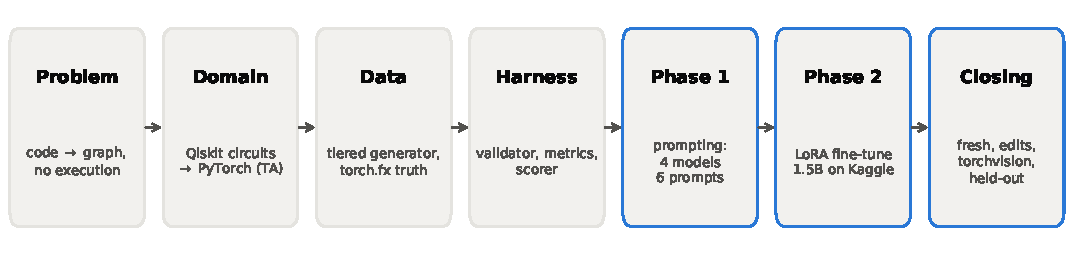
\includegraphics[width=\textwidth]{workflow}
	\caption{Project workflow, from the problem statement to the closing experiments.}\label{fig:workflow}
\end{figure}
How we travelled through this project:
\begin{enumerate}
	\item Plan of action
	\item Mid-term Prep Review 
	\begin{itemize}
		\item Initially started off with a qiskit quantum circuit DAG graphArt idea
		\item Built the script generation, and evaluation pipeline for these DAGs 
	\end{itemize}
	\item Correction after the prep review 
	\begin{itemize}
		\item Shifted focus to the required Deep Neural Network forward pass graph building
		\item Data generation and evaluation had to be rebuilt (viewpoint changes on the already built ones)
	\end{itemize}
	\item Phase 1 prompting on various viable models
	\item Phase 2 LoRA fine tuning 
	\item Imporant checks and out of generated - torchvision testing and realizations
	\item Putting it all together in the requested format
\end{enumerate}

\section{Literature Survey} \label{sec:litsurvey}
% FACT SHEET -- literature survey ("comprehensive survey of at least two or three" papers)
%  READ THESE YOURSELF and summarise in your own words -- the rules give zero for AI-written
%  paper summaries. Pick 3-5. Why each is relevant (one line each):
%  - reed2022torchfx      : where our ground truth comes from; what symbolic tracing records
%  - fatemi2024talklikegraph, wang2023nlgraph : how LLMs read/write graphs as text
%  - gu2024cruxeval, zaremba2014execute, nye2021scratchpad : LLMs predicting what code does;
%    scratchpad/simulation = the idea behind our CoS prompt
%  - wei2022cot, brown2020gpt3 : chain-of-thought (our cot control) and few-shot prompting
%  - hu2022lora (+ dettmers2023qlora) : the fine-tuning method we used
%  - hui2024qwencoder, gemma2025gemma3 : the model families we evaluated
%  - how OUR work differs: exact structural grading, controlled difficulty, edit-based probe
LLMs reading and writing graphs as text - \citep{fatemi2024talklikegraph}, 
Accuracy depends on how a graph is encoded as text; LLMs struggle once graph tasks need multi-step reasoning
You choose one fixed text encoding and grade it exactly; the graph has to come out of code, not out of a description

Throughout the project, we have mostly experimented with the natural direciton of the problem and honestly, did 
not rely and take much inspiration from established literature. This could be one of our many wrong choices but 
this decision was not made out of indifference to the problem.

\section{Proposed Approach or Approaches} \label{sec:our_proj}

\subsection{Work done before prep-presentation review}
% FACT SHEET -- before the prep review
%  - domain: Qiskit circuit DAGs; ground truth from qiskit circuit_to_dag
%  - built: tiered circuit generator, DAG text schema, structural validator,
%    metrics (valid / exact / node F1 / edge F1), prompting pipeline, prep deck
%  - lesson carried over: compare GRAPHS (isomorphism), not operation lists
Before the prep-presentation (midterm) review;
\begin{itemize}
	\item A complete pipeline for generating and evaluating a tiered qiskit circuit generator. 
	\item The ground truth was pulled from qiskit's built in \texttt{<circuit\_to\_dag>} function. 
	\item As mentioned the generator created circuits with multiple levels of ``difficulty'' - basically 
hiding more and more code with the higher levels. 
	\item A common schema was developed for isomorphing, the LLM's generated graph to qiskit's standards. 
	\item Validators were needed to confirm that the LLM produced a real / viable graph. 
	\item The metrics (valid / exact / node F1 / edge F1) were decided upon and the complete prompting pipeline was built with standard prompting techniques.
\end{itemize}
 Nothing else was run or built.

\subsection{Work done after prep-presentation review}
% FACT SHEET -- after the prep review (the bulk of the report)
%  Task formulation
%   - input: Python source defining an nn.Module + example_input; output: graph text
%     (INPUTS / NODES "<id> <op> <target> [Class(params)] [shape]" / EDGES "a -> b : argK")
%   - edges carry ARGUMENT SLOTS (order-sensitive ops); one edge per (src,dst) listing all slots
%  Ground truth + validation (graphart/extract.py, validate.py)
%   - torch.fx symbolic_trace + ShapeProp; function aliases normalised (x+y, torch.add, x.add -> add)
%   - validator checks a reply WITHOUT the answer: acyclic, one output, reachability, arities,
%     module-path tree, shape consistency
%  Metrics (graphart/metrics.py): valid; exact = labelled isomorphism (networkx, VF2);
%     topo = exact ignoring module parameters and function-vs-method spelling (added after the first
%     reply failed on notation, not structure); node/edge F1 on label multisets; shapes scored separately
%  right graph (added after the closing runs, applied to EVERY run, scorer itself unchanged):
%     topo, also forgiving an activation written as a function where the code has a layer (or the
%     reverse), F.max_pool2d vs max_pool2d, and a+b vs b+a; still needs every operation + connection
%  Error classifier (scripts/classify_errors.py): one category per reply by isomorphism tests in a
%     fixed order -- right graph (exact/notation/spelling/commutative), narrow error (arg_slots;
%     coarse_* = a block drawn as one box, checked by RE-TRACING the real code with that block kept
%     whole), wrong (gave_original/miswired/wrong_ops/unparseable). Re-trace reproduces 274/274 stored
%     truths; 11/11 constructed test cases land in the right category; per-reply CSVs in results/errors/
%  Approach A -- prompting (6 prompts, prompts/*.txt): zero_shot, few_shot (3 train examples),
%     cot (control), cos = chain-of-simulation (OURS: interpret forward() line by line, track which node
%     each variable points to), nodes_only / edges_only (decomposition)
%  Approach B -- LoRA fine-tuning (scripts/train_lora.py)
%   - base: Qwen2.5-Coder-1.5B-Instruct, decoder-only transformer, 1.56B params
%   - LoRA on q,k,v,o,gate,up,down projections, r=16, alpha=32, dropout 0.05 -> 18.5M trainable (1.18%)
%   - loss: token cross-entropy on the ANSWER tokens only (prompt masked with label -100) -> Eq. (1)
%   - why LoRA: fits one 16 GB T4; why masking: learn to answer, not to recite the prompt
After the review; task reformulated as: 
\begin{itemize}
	\item input : Python source defining an nn.Module + example\_input; and output : graph\_text
	\item Ground truth: use torch.fx symbolic\_trace + ShapeProp; 
	\item Validation: Checks for desired replies: acyclic, one output, reachability, arities,
	module-path tree, shape consistency
	\item Metrics (graphart/metrics.py): valid; exact = labelled isomorphism; 
	topo = exact ignoring module parameters and function-vs-method spelling;
	node/edge F1 on label multisets; shapes scored separately as a `right graph'.
	\item Error classifier: for precise reasoning of the error / mistake
	\item Phase 1: Prompting : zero\_shot, few\_shot, cot, cos = chain-of-simulation (interpret forward() line by line,
	track which node each variable points to), nodes\_only / edges\_only (decomposition).
	\item Phase 2: LoRA fine-tuning; performed on the smallest Qwen2.5-Coder-1.5B-Instruct,  
	decoder-only transformer, 1.56B params fusing Kaggle's free GPU access.
\end{itemize}

% Equations for Approach B (keep, explain each symbol in your text):
%\begin{align}
%	h &= W_0 x + \frac{\alpha}{r} B A x, \qquad A \in \R^{r \times k},\; B \in \R^{d \times r},\; B_{\text{init}} = 0 \label{eq:lora}\\
%	\mathcal{L}(\theta) &= -\frac{1}{|\mathcal{A}|} \sum_{t \in \mathcal{A}} \log p_\theta\left(y_t \mid y_{<t}, x\right) \label{eq:loss}
%\end{align}

\subsection{Test interface}
% FACT SHEET -- interface (deliverable: "proper methodology for preparing the interface")
%  - what: local web app, interface/app.py (Gradio 6.30); run: .venv/Scripts/python interface/app.py,
%    open http://127.0.0.1:7860; deps in requirements-interface.txt
%  - inputs: paste code, upload a .py file, pick one of 254 examples (40 test, 21 torchvision, 193
%    edits), or GENERATE a fresh program with the project's generator (tier + seed)
%  - pipeline per request: (1) reference = torch.fx trace of the code (graph_from_code; for examples,
%    the stored truth); (2) prediction = the fine-tuned 1.5B (HFBackend + LoRA, zero-shot prompt,
%    greedy) live on CPU (~2 min; 124 s measured), or the answer saved during the experiments for
%    examples (instant); (3) parse with the same parameter-stripping retry as `topo`; (4) score with
%    the project's own compare() + classify(); (5) draw with compare_figure (red = missed,
%    orange = invented)
%  - outputs: side-by-side graphs, 8 metrics (exact, topo, right graph, node F1, edge F1, reach F1,
%    shape accuracy, validity), the error category, validator messages, raw graph text
%  - generated programs are checked against all 1,280 training graphs (Weisfeiler-Lehman hash under
%    the exact-match labels) and the app says whether the graph is new -- so a perfect answer on a
%    generated program can be told apart from recall
%  - design choices: same code path as the experiments (no separate demo logic) so the interface shows
%    exactly what was measured; saved answers make the demo instant; a larger "pensive" model was
%    dropped: Qwen 14B needs ~10 GB free RAM (laptop: 16 GB total), free Gemma endpoint rate-limited
%  - safety: tracing executes the pasted code's constructor -> bound to 127.0.0.1 only
\begin{itemize}
	\item Multiple input methods: paste code, upload a .py file, pick one of 254 examples (40 test, 21 torchvision, 193
    edits), or GENERATE a fresh program with the project's generator (tier + seed).
	\item Reference: torch.fx trace of the code
	\item Prediction: the fine-tuned 1.5B - (easiest on my cpus)
	\item Draw the final graphs and run the comparison, ouputs side by side graphs, 8 metrics etc.
\end{itemize}

\section{Data set Details} \label{sec:data}
% FACT SHEET -- data (README "Dataset" has the tier table)
%  - fully synthetic, text (Python source -> graph text); generator graphart/generate.py; builder
%    scripts/build_dataset.py --per-tier 400 (seed 0 reproduces it)
%  - 4 tiers by how much the code HIDES the graph: T1 flat, T2 loops/Sequential/ModuleList,
%    T3 branches (residual, concat, dead branch, reused layer), T4 blocks (residual CNN, inception,
%    transformer, U-net); nodes T1 7/10.1/14, T2 8/10.4/13, T3 8/12.0/16, T4 12/15.1/25
%  - 1600 programs, 80/10/10 per tier -> 1280 / 160 / 160; dedup by graph text
%  - style randomised separately from structure (14 class names, 5 model variable names,
%    4 import blocks, naming schemes, functional vs module activations) -> against house-style shortcuts
%  - token length (Qwen tokenizer, zero-shot prompt + answer): mean 1400, max 2330
%  - evaluation subsets: stratified 40 (10/tier) for every run; fresh 20 (unused seed);
%    closing: torchvision 21 (real source, 18 blocks + alexnet/squeezenet1_1/resnet18),
%    edits 193 (124 neutral, 69 meaningful), rq6 probe 84
%  - found later: dedup by TEXT let 4/160 test graphs duplicate a train graph (other node order);
%    1 in the scored 40 (t4-00340); left in place for comparability, reported
%  - what the generator never varies (counted over the 1280 training programs vs the 21 torchvision):
%    own block classes 0 vs 10; grouped convs 0 vs 5; tuple kernels 0 vs 3; un-shortened F.
%    functions 0 vs 7; the input is ALWAYS called x (1280/1280); every `if self.<flag>:` branch has
%    the flag False (168/168, none True). It varies how code is SPELLED, not how it is ORGANISED.
%  - torchvision split, fixed by a mechanical rule BEFORE the tuned model's results were opened:
%    in-distribution 5 (none of the constructs above, no assert) / unseen 16.
%    DISCLOSE: the rule missed helper FUNCTIONS (conv3x3/conv1x1, all 3 ResNet samples) and the input
%    name (MNASNet uses `input`); split kept as fixed
%  - rq6 probe 84 = control 22, dead_branch 18, dead_flag 40 (dead `if` added), branch_on 4 (flag True)
%  - EXTRACTION, step by step (data procurement):
%    synthetic: scripts/build_dataset.py --per-tier 400 (seed 0): generate -> exec -> torch.fx trace +
%      ShapeProp -> validate -> dedup -> stratified 80/10/10 split per tier -> data/generated/*.jsonl
%    torchvision (scripts/build_torchvision_set.py): for each block, pull torchvision's OWN source with
%      `inspect` (the class + the helpers it uses + imports), append one construction line and an
%      example input, trace it, and check the graph is isomorphic to tracing the genuine torchvision
%      object -- so the assembled code is known to define exactly torchvision's graph (21/21 pass)
%    edits (scripts/build_edit_set.py): programmatic edits of the 40 test programs; each re-traced, and
%      a meaningful edit is kept only if its graph differs from the original's (0 violations checked)
%    rq6 (scripts/build_rq6_probe.py): test programs grouped by construct + the dead_flag/branch_on edits
%    source: github.com/pytorch/vision (torchvision 0.x source, cite web_torchvision); all data is
%      text (Python source + graph text); data/generated/ is in the repository
\begin{table}[!h]
\centering
\small
\begin{tabular}{lcccccc}
\hline
Tier & programs & train & val & test & nodes min / mean / max & merges / graph \\
\hline
1 flat & 400 & 320 & 40 & 40 & 7 / 10.1 / 14 & 0.00 \\
2 loops & 400 & 320 & 40 & 40 & 8 / 10.4 / 13 & 0.00 \\
3 branches & 400 & 320 & 40 & 40 & 8 / 12.0 / 16 & 2.02 \\
4 blocks & 400 & 320 & 40 & 40 & 12 / 15.1 / 25 & 1.88 \\
all & 1600 & 1280 & 160 & 160 &  &  \\
\hline
\end{tabular}
\caption{The synthetic data set: four tiers by how much the code hides the graph. A merge is a node with more than one incoming value (residuals, concatenations).}\label{tab:data}
\end{table}

\begin{itemize}
	\item Fully synthetically generated using a builder script.
	\item 4 tiers by how much the code HIDES the graph: T1 flat, T2 loops/Sequential/ModuleList,
    T3 branches (residual, concat, dead branch, reused layer), T4 blocks (residual CNN, inception,
    transformer, U-net); 
\end{itemize}

\section{Experiments} \label{sec:exp}

\textcolor{red}{The team should include all experiments, even those with negative results, and address all experiments that were performed.}

% FACT SHEET -- experiments
\begin{itemize}
	\item Hardware: laptop (Windows, Intel Iris Xe, CPU only) for local runs; Kaggle 2x NVIDIA T4 16 GB (training uses one); OpenRouter free tier (50 requests/day) for Gemma
	\item Models: Qwen2.5-Coder 1.5B / 7B / 14B (Ollama, 4-bit), Gemma 4 31B (OpenRouter), 1.5B fp16 (HF)
	\item Decoding: greedy / temperature 0; 1500-token cap (4096 for cot/cos, 3200 for torchvision); Ollama num\_ctx 8192, think=false
	\item Training (Phase 2): HF Trainer, AdamW (fused, default betas), lr 2e-4, cosine schedule, 3\% warmup, 2 epochs = 160 steps, effective batch 16 (1 x 16 accumulation), max length 2560, fp16, gradient checkpointing, seed 0, val loss every 40 steps, best checkpoint kept; 97.5 min val loss 0.0016 $\rightarrow$ 0.0003 $\rightarrow$ 0.00009 $\rightarrow$ 0.00009
	\item Negative results / problems (template asks for ALL experiments):
	\begin{itemize}
		\item first reply failed to parse: prompts defined labels for 2 of 14 layer types $\rightarrow$ label table + topo
		\item cos prompt lacked the Sequential rule $\rightarrow$ re-run; did not improve tier 2
		\item free OpenRouter endpoint $\sim$1 reply / 15-20 min $\rightarrow$ moved to Kaggle
		\item Gemma 4 ``thinking'' returned empty replies $\rightarrow$ think=false
		\item two Kaggle fine-tuning failures: 35 examples $>$ 2048 tokens; Kaggle's old torchao vs peft
	\end{itemize}
	\item Speeds measured on T4: tuned 1.5B $\sim$24 tok/s, Qwen 7B $\sim$34, Qwen 14B $\sim$16; Gemma $\sim$5
	\item Closing runs (each capped at 2.5 h of Kaggle time): Qwen 14B zero-shot via Ollama on torchvision + edits; tuned 1.5B (HF, greedy) on torchvision + edits + rq6; held-out adapter trained WITHOUT any dead-branch program (1112 examples, ONE epoch = 70 steps, 43 min, same hyper-parameters otherwise) and run on rq6. No reply truncated (all have their edge list).
	\item think=false: matters only for models with a thinking mode (Gemma 4 returned empty replies, 288 s for 0 characters); Qwen2.5-Coder has none, so it changed nothing for any Qwen run
\end{itemize}


\section{Results}\label{sec:results}
% FACT SHEET -- results (figures + tables below; inference text is yours)
%  RQ1 scale/tiers (Fig scale, Tab scale): chains before branches; 7B 0/20 on T3-T4; branching from 14B
%  RQ2 decomposition (Tab prompts): nodes_only 0.70, edges_only 0.75, full 0.60 ~ 0.70 x 0.75;
%     both break on T3 (0.40 each) -> no extra cost for doing both at once
%  prompts (Fig prompts): cot 0.53 < zero_shot 0.60; cos best on T3 (7/10 vs 1-4/10) but weak on
%     T2 containers (extra Sequential node / one-level nesting); 14B "[]" format slip in 18/40
%  why CoT/CoS did not simply win (right graph per tier, of 10: zero 10/10/4/4=28, few 10/10/5/6=31,
%     CoS 10/3/7/7=27, CoT 9/9/3/3=24): CoS best on T3+T4 (14/20 vs few 11, zero 8) -- tracing is
%     what those tiers need -- but collapses on T2; without T2 CoS leads 24/30 vs 21/30. CoT worse
%     everywhere: reply 2.4x longer (median 1652 vs 698 chars), no task procedure, more format drift
%     (8 unreadable vs 4); CoT gains reported at far larger scale, short-answer tasks (wei2022cot).
%     Few-shot wins by FORMAT: raw parse failures 21 -> 4, exact 7 -> 19. 10/tier: T2 collapse real,
%     T3/T4 lead suggestive only
%  Gemma misses: all notation (x.tanh as function, 7) or tuple-unpacking getitem (3 transformers)
%  RQ3 (Fig finetune, Tab finetune): LoRA 1.5B 40/40 exact; untuned 0/40; Gemma 30/40 exact, 37/40 topo
%  leak audit: no answer in prompts; train/val only; 0 identical programs/answers; 0 replies copy a
%     training answer; same scorer gives untuned 0/40; 1/40 isomorphic duplicate -> 39/39
%  fresh programs: 20/20 exact (unused seed, none isomorphic to any split)
%  Right-graph column (Tabs scale/prompts/finetune): ranking never changes, gaps do -- LoRA 40 vs
%     Gemma 37 (vs 40 vs 30 on exact); 7B 10 -> 17. The untuned 1.5B is 4/40 even with spelling
%     forgiven: invents layers, drops them, draws Sequential as one box -> it could NOT read the code
%  RQ4 real code (Fig closing, Tab closing_rq4): right graph 14B 4/21, LoRA 0/21; in-distribution
%     14B 4/5, LoRA 0/5; unseen 0/16 both. LoRA draws 16 of its 18 readable replies as ONE STRAIGHT
%     CHAIN (only 4 of 21 truths are chains; on our test it does so 0 of 18 times): SqueezeNet Fire
%     loses its branch and cat, ResNet BasicBlock loses the skip and gains a `downsample` conv that is
%     None in the code. 14B: 2 of 14. 14B failures: 7 unparseable (broke stated rules for g= and k=[..]
%     in situations never exemplified), 3 spelling-only (relu as function), 3 coarse (block as a box)
%  RQ5 edits (Tab closing_rq5), programs each model solved first (14B 24, LoRA 40): neutral right
%     87% / 94%; meaningful right 22% / 25%; meaningful answered with the UNEDITED graph 64% / 68%;
%     reroute followed 0/14 / 0/27; swap cat 0/4 / 0/9; drop call 8/18 / 17/29. Spot-checked by hand
%     (fc1(h) -> fc1(x): reply keeps the old h -> fc1 edge). Reorder: of 13, 7 only swap + operands
%     (same computation; strict exact counts it wrong), 6 put cat inputs in written order
%  RQ6 held-out (Tab closing_rq6): held-out adapter dead branch 2/18, writes the dead layer in 18/58;
%     full adapter 18/18 BUT deletes the layer when the flag is True, 0/4 -- training never had a True
%     flag, so "delete what is under if self.flag" was a correct rule on that data
%  Answer to "rule or generator?": mostly the generator. Real reading within the family (40/40,
%     20/20 fresh, untuned 4/40) but leaning on shortcuts the data allowed; as a reader of code in
%     general the tuned 1.5B is weaker than the prompted 14B. The edit signature is SHARED by the 14B,
%     so not caused by fine-tuning. Caveats: n=4 flag-True, n=5 in-distribution, one seed, held-out
%     adapter 1 epoch vs 2 (control 1.00 -> 0.86 partly that), all-160 re-score not run
\begin{figure}[!h]
	\centering
	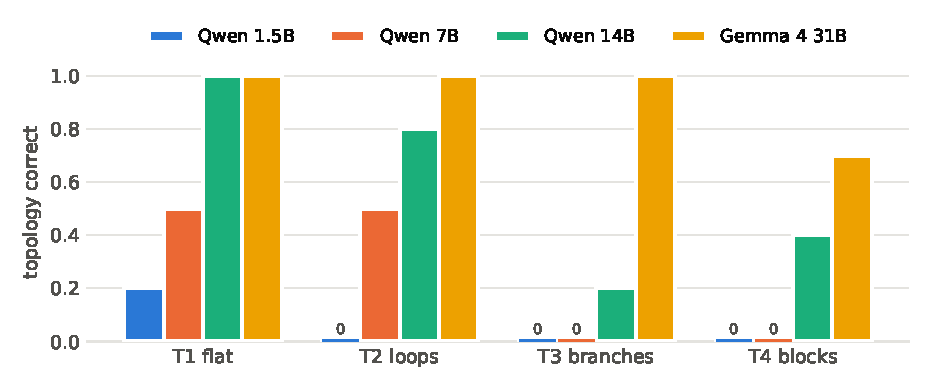
\includegraphics[width=\textwidth]{scale_by_tier}
	\caption{Zero-shot: share of the 40 test programs with the correct topology, by tier and model size.}\label{fig:scale}
\end{figure}
\begin{table}[!h]
\centering
\small
\begin{tabular}{lcccccccc}
\hline
Model (zero-shot) & T1 & T2 & T3 & T4 & topo & exact & right graph & parsed \\
\hline
Qwen 1.5B & 0.20 & 0.00 & 0.00 & 0.00 & 0.05 & 0.00 & 0.07 & 0.62 \\
Qwen 7B & 0.50 & 0.50 & 0.00 & 0.00 & 0.25 & 0.20 & 0.42 & 0.80 \\
Qwen 14B & 1.00 & 0.80 & 0.20 & 0.40 & 0.60 & 0.17 & 0.70 & 0.47 \\
Gemma 4 31B & 1.00 & 1.00 & 1.00 & 0.70 & 0.93 & 0.75 & 0.93 & 0.93 \\
\hline
\end{tabular}
\caption{Zero-shot accuracy by model size on the 40 stratified test programs (10 per tier). Tier columns and \emph{topo} count graphs with the right topology; \emph{exact} is strict; \emph{right graph} also forgives spelling that does not change the computation.}\label{tab:scale}
\end{table}


\begin{figure}[!h]
	\centering
	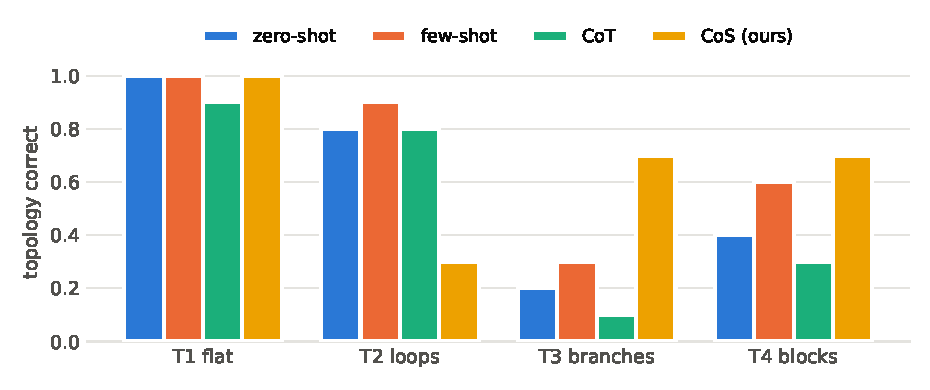
\includegraphics[width=\textwidth]{prompts_by_tier}
	\caption{Prompting strategies on Qwen2.5-Coder 14B, by tier (topology correct).}\label{fig:prompts}
\end{figure}
\begin{table}[!h]
\centering
\small
\begin{tabular}{lcccccccc}
\hline
Prompt (Qwen 14B) & T1 & T2 & T3 & T4 & topo & exact & right graph & parsed \\
\hline
zero-shot & 1.00 & 0.80 & 0.20 & 0.40 & 0.60 & 0.17 & 0.70 & 0.47 \\
few-shot & 1.00 & 0.90 & 0.30 & 0.60 & 0.70 & 0.47 & 0.78 & 0.90 \\
CoT & 0.90 & 0.80 & 0.10 & 0.30 & 0.53 & 0.15 & 0.60 & 0.55 \\
CoS (ours) & 1.00 & 0.30 & 0.70 & 0.70 & 0.68 & 0.30 & 0.68 & 0.62 \\
nodes only & 1.00 & 0.80 & 0.40 & 0.60 & 0.70 & 0.17 & -- & 0.47 \\
edges only & 1.00 & 1.00 & 0.40 & 0.60 & 0.75 & 0.75 & -- & 1.00 \\
full task & 1.00 & 0.80 & 0.20 & 0.40 & 0.60 & 0.17 & 0.70 & 0.47 \\
\hline
\end{tabular}
\caption{Prompting strategies and the read/wire decomposition on Qwen2.5-Coder 14B, same 40 programs. \emph{right graph} applies to whole-graph replies only.}\label{tab:prompts}
\end{table}


\begin{figure}[!h]
	\centering
	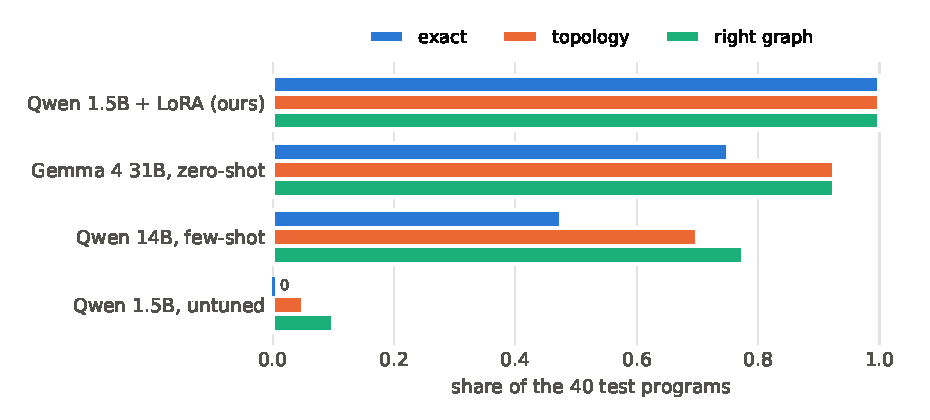
\includegraphics[width=\textwidth]{finetune_vs_prompting}
	\caption{The LoRA-tuned 1.5B against its untuned base and the best prompted models.}\label{fig:finetune}
\end{figure}
\begin{table}[!h]
\centering
\small
\begin{tabular}{lccccc}
\hline
Model & exact & topo & right graph & reach F1 & parsed \\
\hline
Qwen 1.5B, untuned & 0.00 & 0.05 & 0.10 & 0.32 & 0.75 \\
Qwen 14B, few-shot & 0.47 & 0.70 & 0.78 & 0.88 & 0.90 \\
Gemma 4 31B, zero-shot & 0.75 & 0.93 & 0.93 & 0.93 & 0.93 \\
Qwen 1.5B + LoRA (ours) & 1.00 & 1.00 & 1.00 & 1.00 & 1.00 \\
\hline
\end{tabular}
\caption{Fine-tuning against prompting, same 40 test programs and the same zero-shot prompt for the two 1.5B rows. All on our generator's programs; Table~\ref{tab:closing_rq4} has real code.}\label{tab:finetune}
\end{table}


\begin{figure}[!h]
	\centering
	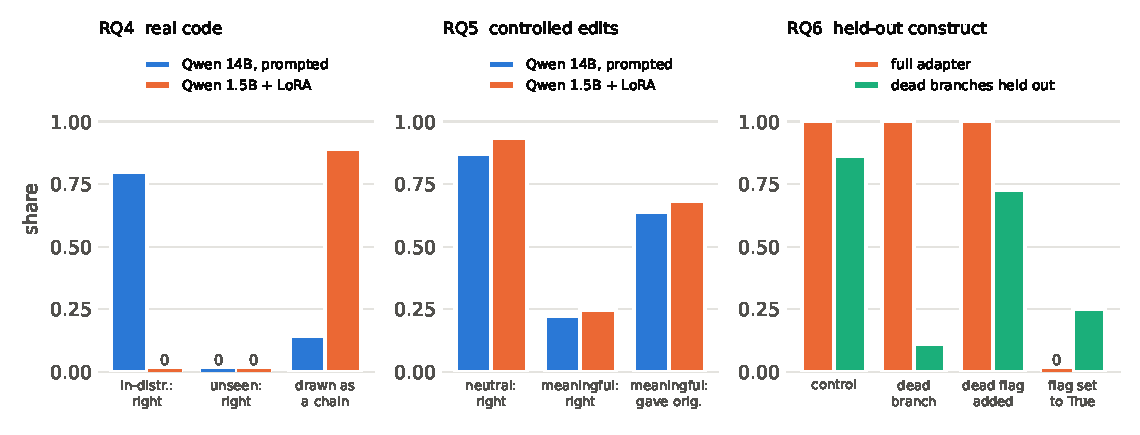
\includegraphics[width=\textwidth]{closing}
	\caption{Closing experiments. RQ4: torchvision, right graph on in-distribution and unseen-construct samples, and the share of readable replies drawn as one straight chain. RQ5: controlled edits on programs each model solved first. RQ6: the full adapter against one trained without dead branches.}\label{fig:closing}
\end{figure}
\begin{table}[!h]
\centering
\small
\begin{tabular}{lccccccccc}
\hline
torchvision (21) & parsed & exact & topo & right & node F1 & edge F1 & in-distr. & unseen & chain \\
\hline
Qwen 14B, prompted & 14 & 1 & 1 & 4 & 0.31 & 0.20 & 4 / 5 & 0 / 16 & 2 / 14 \\
Qwen 1.5B + LoRA & 18 & 0 & 0 & 0 & 0.36 & 0.17 & 0 / 5 & 0 / 16 & 16 / 18 \\
\hline
\end{tabular}
\caption{RQ4, real code: counts over 21 torchvision samples. \emph{In-distr.} (5 samples) have none of the constructs absent from all 1,280 training programs (own block classes, grouped convolutions, tuple kernels, un-shortened \texttt{F.} functions, \texttt{assert}); the rule was fixed before the tuned model's results were opened. \emph{Right} is the right-graph level. \emph{Chain}: readable replies with no branch at all; 4 of the 21 true graphs are chains.}\label{tab:closing_rq4}
\end{table}

\begin{table}[!h]
\centering
\small
\begin{tabular}{lccccccc}
\hline
edits & solved & neutral & meaningful & gave original & reroute & swap cat & drop call \\
\hline
Qwen 14B, prompted & 24 & 61 / 70 & 8 / 36 & 23 / 36 & 0 / 14 & 0 / 4 & 8 / 18 \\
Qwen 1.5B + LoRA & 40 & 116 / 124 & 17 / 69 & 47 / 69 & 0 / 27 & 0 / 9 & 17 / 29 \\
\hline
\end{tabular}
\caption{RQ5, controlled edits of the test programs, counting only the programs each model got right before the edit (\emph{solved}). Columns count right graphs, except \emph{gave original}: meaningful edits answered with the graph of the unedited program.}\label{tab:closing_rq5}
\end{table}

\begin{table}[!h]
\centering
\small
\begin{tabular}{lccccc}
\hline
rq6 probe (84) & control & dead branch & dead flag added & flag True & dead layer in \\
\hline
full adapter & 22 / 22 & 18 / 18 & 40 / 40 & 0 / 4 & 0 / 58 \\
dead branches held out & 19 / 22 & 2 / 18 & 29 / 40 & 1 / 4 & 18 / 58 \\
\hline
\end{tabular}
\caption{RQ6, a held-out construct: the full adapter against one trained without any dead-branch program (1,112 examples, one epoch against two). Group columns count topology-correct graphs. All 168 flagged branches in the training data have the flag \texttt{False}.}\label{tab:closing_rq6}
\end{table}


% Qualitative results (scripts/make_report_figures.py, fig_qualitative): red = in the reference,
% missed; orange = invented by the model.
%  - fig:qual_14b: 14B zero-shot writes in a dead branch (fc2 under `if self.wide:` with wide=False),
%    renames a reused layer (fc3 -> invented fc3_1), and spells sigmoid as a function
%  - fig:qual_chain: the tuned 1.5B on SqueezeNet's Fire block: both branches chained, cat dropped
%  - fig:qual_reroute: the tuned 1.5B on an edit fc1(h) -> fc1(x): it keeps the old flat1 -> fc1
%    edge and misses x -> fc1 -- the "gave the original graph" signature
\begin{figure}[!h]
	\centering
	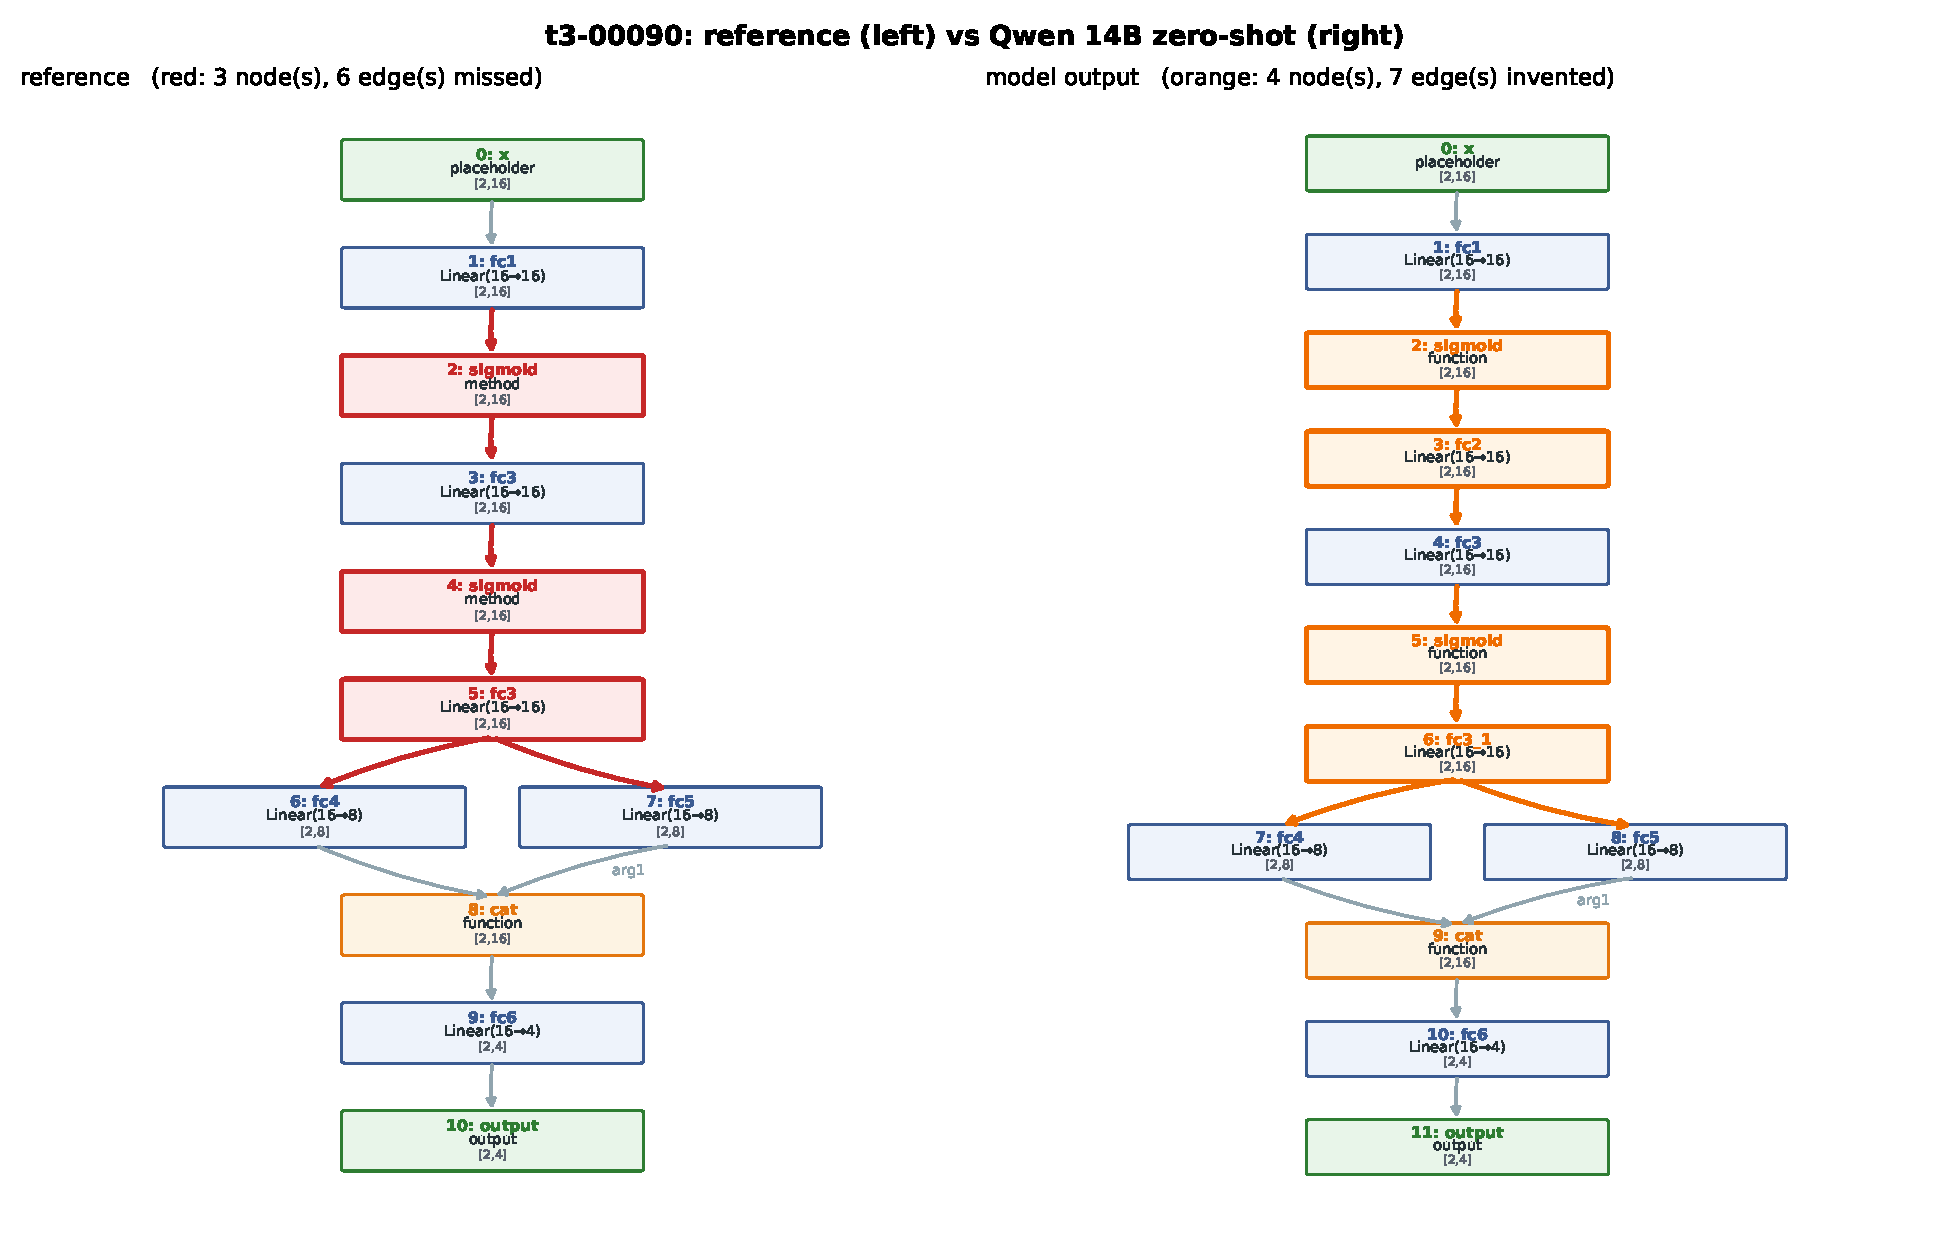
\includegraphics[width=\textwidth]{qual_14b_dead_branch}
	\caption{Qualitative: Qwen 14B zero-shot on a tier-3 test program. Red: in the reference, missed; orange: invented.}\label{fig:qual_14b}
\end{figure}
\begin{figure}[!h]
	\centering
	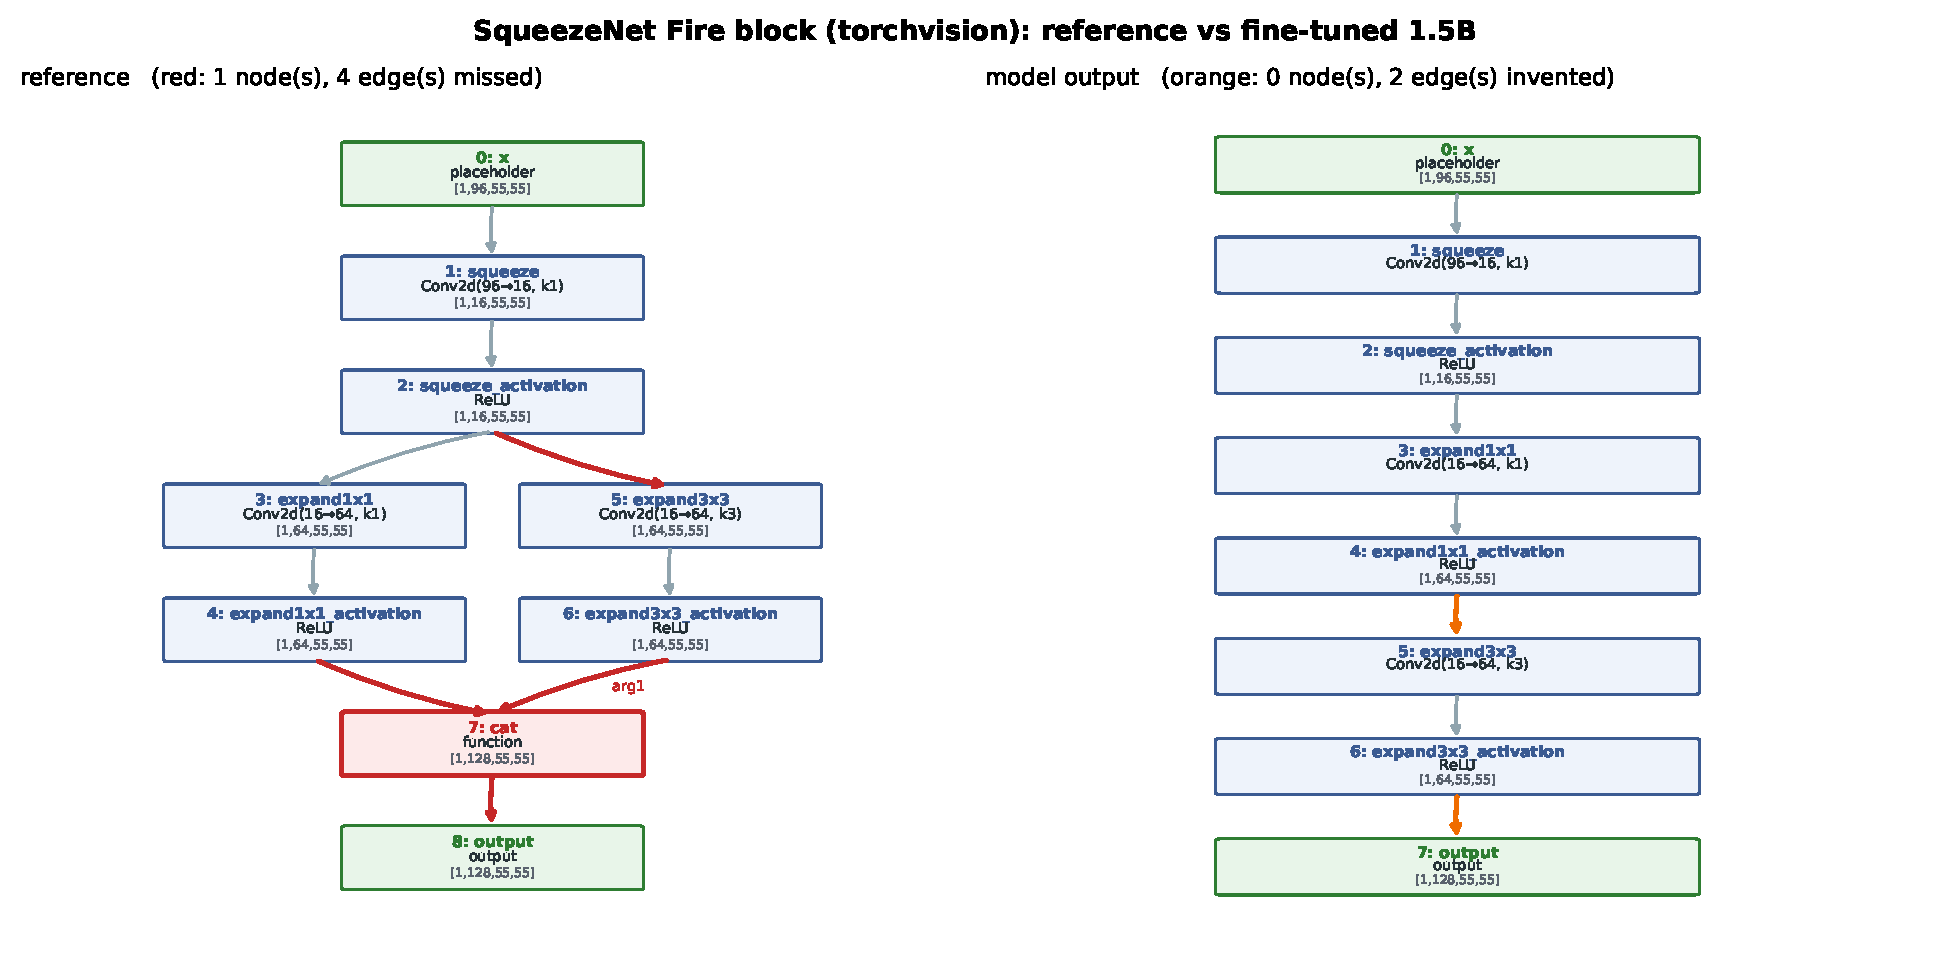
\includegraphics[width=\textwidth]{qual_lora_chain}
	\caption{Qualitative: the fine-tuned 1.5B on torchvision's SqueezeNet Fire block draws a chain.}\label{fig:qual_chain}
\end{figure}
\begin{figure}[!h]
	\centering
	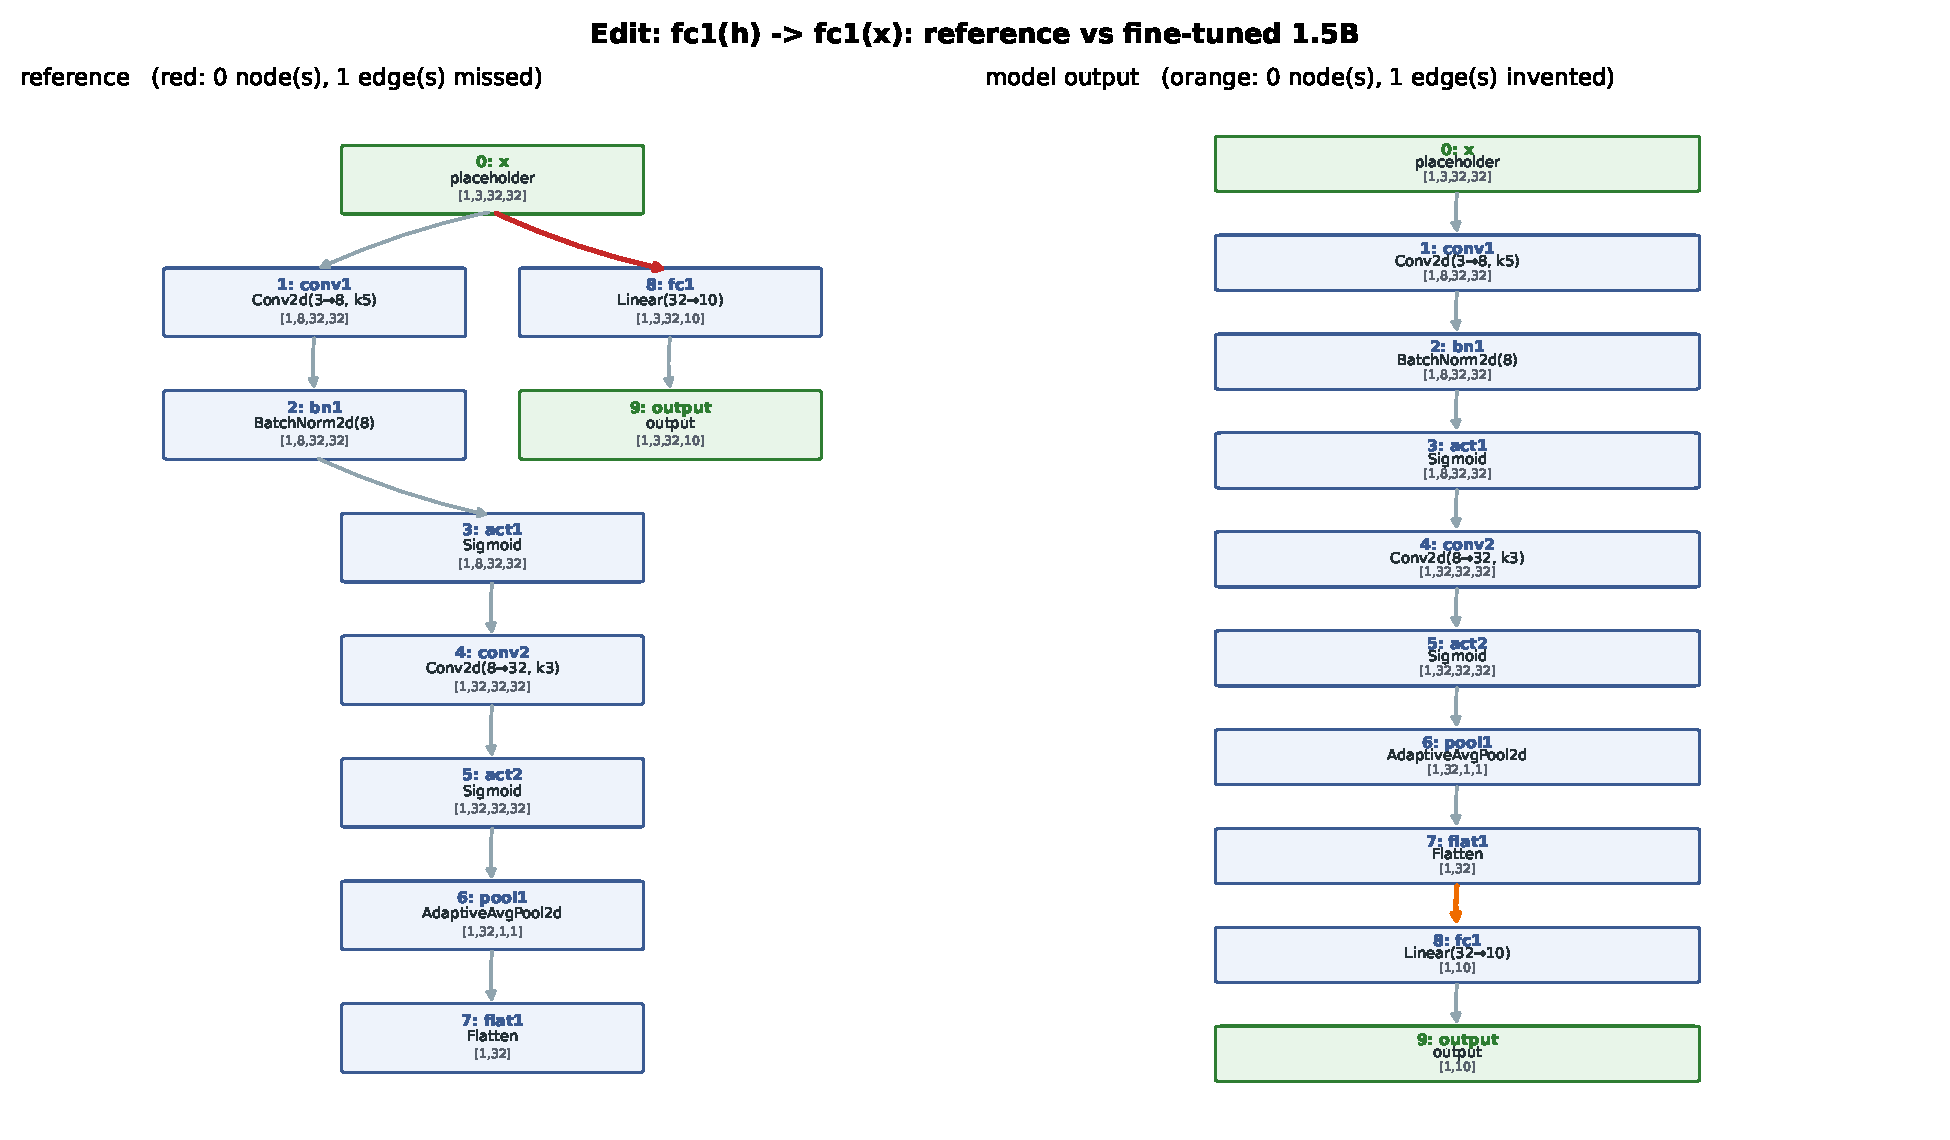
\includegraphics[width=0.85\textwidth]{qual_lora_reroute}
	\caption{Qualitative: the fine-tuned 1.5B on a rerouted input answers with the unedited graph.}\label{fig:qual_reroute}
\end{figure}
\begin{itemize}
	\item (RQ1)Zero-shot topology climbs with size:
		1.5B: 0.05
		7B: 0.25
		14B: 0.60
		Gemma 31B: 0.93
	\item (RQ1)Chains come before branches. The 7B gets 0 on tiers 3–4; 
	branching first appears at 14B (T3 0.20, T4 0.40); 
	Gemma solves tier 3 completely (1.00).
	\item (RQ2) Decomposition:
	reading alone (nodes only): 0.70
	wiring given nodes (edges only): 0.75
	both at once: 0.60
	\item (RQ2) Prompts: CoT: 0.53, below zero-shot (0.60). 
	Its replies are about 2.4× longer (median 1,652 vs 698 characters) and drift from the format more.
	Few-shot: best overall at 0.70, mostly by fixing format. Raw parse failures fall 21 → 4, exact rises 7 → 19.
	CoS: best on the hard tiers, but collapses on loops. Therefore, we infer that structured simulation helps where 
	reasoning is the bottleneck; and giving examples clears out the format.
	\item (RQ3) Fine-tuning (1.87 percent): LoRA 1.00 on every metric for the worst performing 1.5B model.
	Found it a little suspicious at first, so audited it for any leakage of information, and so 
	tested with 20 newly generated programs - still scored perfectly.
	\item Outside the Generators: THe real test and the real performance on real torchvision codes
	LoRA performs poorly, worse than the zero shot prompted 14B model; but a better Reach F1. So it's clear 
	that LoRA fine tuned 1.5B simply memorised shortcuts for the house style generated code. 
\end{itemize}

\FloatBarrier
\section{Plan for Novelty Assessment} \label{sec:Plan for Novelty Assessment}
% FACT SHEET -- novelty plan (assessment 23/25 Nov)
%  - what is already new: chain-of-simulation prompt; read/wire decomposition; edit-based probe of
%    "understanding" (neutral vs meaningful edits, "answered the original graph" signature);
%    held-out-construct fine-tuning
%  - the closing runs say what to fix first: remove the shortcuts the data allowed -- flags that are
%    sometimes True, varied input names, helper classes AND functions, layers outside the menu
%    (grouped convs, tuple kernels) -- retrain, and re-run RQ4-RQ6 to see if the chain/original-graph
%    signatures go; edit-augmented training (pairs that differ only in wiring)
%  - next: Gemma 31B on the edits; all 160 test; length generalisation
%    to whole networks (answers up to ~3000 tokens vs 877 in training); curriculum or chunked output
%    for big graphs; fine-tune with edit-augmented data; (interface: DONE, see the Test interface
%    subsection) -- earlier plan line kept for the record: paste code -> predicted vs
%    reference graph with differences highlighted
The closing experiments did more than measure accuracy: they showed which shortcuts the
fine-tuned model took, and each of them points to a change in the data. The plan for the novelty
assessment is to remove those shortcuts and test whether the model then learns the rule.
\begin{enumerate}
	\item \textbf{Remove the shortcuts from the generator (main idea).} Add flags that are sometimes
	\texttt{True}, varied names for the input, helper classes and helper functions of the kind
	torchvision uses, and layers outside the current menu such as grouped convolutions and non-square
	kernels. Retrain the same LoRA set-up and re-run the three probes. Success means the tuned model
	gets some of the torchvision graphs right (above 0 of 21), answers far fewer meaningful edits with
	the old graph (well below 68\%), and keeps branches whose flag is \texttt{True}.
	\item \textbf{Train on edit pairs.} Add training pairs that differ only in their wiring --- the same
	program with one input rerouted --- so that the answer cannot be produced from the familiar shape
	of the code. Test on the held-out edit set.
	\item \textbf{Firmer numbers.} Repeat the main runs over several training seeds and on all 160 test
	programs, and run the strongest prompted model (Gemma 4 31B) on the edit set, to see whether the
	old-graph answers also appear at larger scale.
\end{enumerate}
Each retraining takes about 100 minutes on a free Kaggle GPU, and the probes, scoring and error
classification already exist, so the plan fits in the time before the assessment.

\section{Conclusion} \label{sec:conclusion}
% FACT SHEET -- conclusion
%  - problem, methods, headline numbers (scale curve; 1.5B+LoRA 40/40 + 20/20 fresh; leak audit)
%  - closing answer: fine-tuning learned the generator's family, with shortcuts (chains on real code,
%    0/27 rerouted inputs, flag never read); both models redraw the familiar graph on edits (64%/68%)
%  - lesson: a perfect in-distribution score + a clean leak audit still did not show understanding;
%    behavioural probes with exact ground truth (edits, held-out constructs, real code) did
%  - significance: exact, free, scalable grading of code->structure understanding
This project asked whether a language model can turn the source code of a PyTorch network into
its forward-pass graph without running it, and whether it understands the structure it draws. Using
\texttt{torch.fx} as an exact answer key, a tiered generator of programs, and a pipeline that grades
replies by graph isomorphism, we compared prompting across four models and six prompts with LoRA
fine-tuning of a small model.

Prompting improves with scale and with the right prompt: topology accuracy rises from 0.05 to 0.93
between 1.5B and 31B parameters, branching code is solved last, and simulating the code line by line
helps on the hardest tiers while worked examples help most with the output format. Fine-tuning a 1.5B
model is enough to solve the task on our generator's programs, including programs it has never seen.

The closing experiments qualify that result. Outside the generator the tuned model fails, and both it
and the prompted 14B answer changed wiring with the graph the code used to have. The model learned to
read code from one family, together with shortcuts that family allowed. The broader lesson is about
evaluation: a perfect score on held-out data and a clean leak audit were not evidence of
understanding, while small controlled probes with exact ground truth were. Removing those shortcuts
from the data, and testing again, is the next step.

\section*{Code}
The code, data generator, prompts, notebooks and results are available at
\url{https://github.com/Rao-Adarsh/graphArt_LM}.

% Lists every entry while the text has few citations; remove once each source is \citep'd.
\nocite{*}
\bibliographystyle{plain}
\bibliography{references}

\end{document}
